\documentclass[11pt]{article} 
%\usepackage{amsbsy} % for \boldsymbol and \pmb 
%\usepackage{graphicx} % To include pdf files!
\usepackage{amsmath}
\usepackage{amsbsy}
\usepackage{amsfonts}
\usepackage{enumerate}
\usepackage[colorlinks=true, pdfstartview=FitV, linkcolor=blue, citecolor=blue, urlcolor=blue]{hyperref} % For links
\usepackage{fullpage}
\pagestyle{empty}
\usepackage{pgf,pgfplots,tikz}
\usepackage{amsmath,amssymb,amsthm}
\usepackage{tikz}
\newcommand{\overrightharp}[1]{\hat{#1}}
\DeclareMathOperator{\proj}{proj}
\DeclareMathOperator{\years}{years}
\DeclareMathOperator{\cm}{cm}
\newcommand{\vct}{\mathbf}
\newcommand{\vctproj}[2][]{\proj_{{#1}}\vct{#2}}
\newtheorem{theorem}{Theorem}
\DeclareMathOperator{\m}{m}
\DeclareMathOperator{\kg}{kg}
\DeclareMathOperator{\N}{N}
\DeclareMathOperator{\Or}{or}
\DeclareMathOperator{\J}{J}
\DeclareMathOperator{\s}{s}
\DeclareMathOperator{\g}{g}
\DeclareMathOperator{\W}{W}
\DeclareMathOperator{\Heatoms}{He\hspace{1mm} atoms}
\DeclareMathOperator{\MeV}{MeV}
\DeclareMathOperator{\tr}{tr}
\newcommand{\norm}[1]{\left\lVert#1\right\rVert}
\usepackage{graphicx}
\newcommand{\abs}[1]{\lvert#1\rvert}
\DeclareMathOperator{\diverge}{div\,}
\DeclareMathOperator{\curl}{curl\,}
\title{\textbf{PHY325 PS1}
\author{Maxim Piatine\\1005303100}}
\date{}
\DeclareMathOperator{\lineint}{\int \mathbf{v}\cdot d\mathbf{l}}
\DeclareMathOperator{\surfint}{\int \mathbf{v}\cdot d\mathbf{a}}
\begin{document}
\maketitle
\section*{Question 2a}
\begin{center}
$M=\begin{pmatrix}
5 & -4 & 4\\
12 & -11 & 12\\
4 & -4 & 5
\end{pmatrix}$
\end{center}
Using the notes we have in class for eigenvalues:
\[\det (M-\lambda I)\]
\[\det \left( 
\begin{pmatrix}
5 & -4 & 4\\
12 & -11 & 12\\
4 & -4 & 5
\end{pmatrix} -
\begin{pmatrix}
\lambda & 0 & 0\\
0 & \lambda & 0\\
0 & 0 & \lambda
\end{pmatrix}
\right)=\det 
\begin{pmatrix}
5-\lambda & -4 & 4\\
12 & -11-\lambda & 12\\
4 & -4 & 5-\lambda
\end{pmatrix}\]
\[=(5-\lambda)
\det\begin{pmatrix}
-11-\lambda & 12\\
-4 & 5-\lambda
\end{pmatrix}-(-4)
\det\begin{pmatrix}
12 & 12\\
4 & 5-\lambda
\end{pmatrix}+(4)
\det\begin{pmatrix}
12 & -11-\lambda\\
4 & -4
\end{pmatrix}\]
\[=(5-\lambda)((-11-\lambda)(5-\lambda)-(12)(-4))
+4((12)(5-\lambda)-(4)(12))
+4((12)(-4)-(-11-\lambda)(4))\]
\[=(5-\lambda)(\lambda^2+6\lambda-7)
+4(12-12\lambda)
+4(4\lambda-4)=
-\lambda^3-\lambda^2+37\lambda-35+48-48\lambda+16\lambda-16\]
\[=-\lambda^3-\lambda^2+5\lambda-3=-(\lambda-1)^2(\lambda+3)\]
The eigenvalues are $\lambda_{1,2}=1,-3$ where $\lambda_1=1$ has a multiplicity of $2$.\\
Eigenvectors for $\lambda=1$:
\[(M-\lambda_n I)\Vec{\xi}=0\]
\[\left( 
\begin{pmatrix}
5 & -4 & 4\\
12 & -11 & 12\\
4 & -4 & 5
\end{pmatrix} -
\begin{pmatrix}
1 & 0 & 0\\
0 & 1 & 0\\
0 & 0 & 1
\end{pmatrix}
\right)
\begin{pmatrix}
x\\
y\\
z
\end{pmatrix}=0\]
\[=\begin{pmatrix}
4 & -4 & 4\\
12 & -12 & 12\\
4 & -4 & 4
\end{pmatrix}
\begin{pmatrix}
x\\
y\\
z
\end{pmatrix}=
\begin{pmatrix}
1 & -1 & 1\\
0 & 0 & 0\\
0 & 0 & 0
\end{pmatrix}
\begin{pmatrix}
x\\
y\\
z
\end{pmatrix}=0\]
\[x-y+z=0\]
Let $y=s$, $z=t$, and $x=s-t$:
\[\Vec{\xi}=
\begin{pmatrix}
s-t\\
s\\
t
\end{pmatrix}=
\begin{pmatrix}
1\\
1\\
0
\end{pmatrix}s+
\begin{pmatrix}
-1\\
0\\
1
\end{pmatrix}t\]
\[\Vec{\xi_1}=
\begin{pmatrix}
1\\
1\\
0
\end{pmatrix},
\Vec{\xi_2}=
\begin{pmatrix}
-1\\
0\\
1
\end{pmatrix}\]
Eigenvector for $\lambda=-3$:
\[\begin{pmatrix}
8 & -4 & 4\\
12 & -8 & 12\\
4 & -4 & 8
\end{pmatrix}
\begin{pmatrix}
x\\
y\\
z
\end{pmatrix}=
\begin{pmatrix}
2 & -1 & 1\\
3 & -2 & 3\\
1 & -1 & 2
\end{pmatrix}
\begin{pmatrix}
x\\
y\\
z
\end{pmatrix}=
\begin{pmatrix}
1 & 0 & -1\\
3 & -2 & 3\\
1 & -1 & 2
\end{pmatrix}
\begin{pmatrix}
x\\
y\\
z
\end{pmatrix}_{(R1-2R3)}\]
\[=
\begin{pmatrix}
1 & 0 & -1\\
0 & 1 & -3\\
0 & -1 & 3
\end{pmatrix}
\begin{pmatrix}
x\\
y\\
z
\end{pmatrix}_{(R2-3R3),(R3-R1)}=
\begin{pmatrix}
1 & 0 & -1\\
0 & 1 & -3\\
0 & 0 & 0
\end{pmatrix}
\begin{pmatrix}
x\\
y\\
z
\end{pmatrix}_{(R3-R2)}=0\]
\[x-z=0\]
\[y-3z=0\]
Let $z=1$:
\[x=1, y=3\]
\[\Vec{\xi_3}=
\begin{pmatrix}
1\\
3\\
1
\end{pmatrix}\]
Therefore, the eigenvectors are $\begin{pmatrix}
1\\
3\\
1
\end{pmatrix},
\begin{pmatrix}
-1\\
0\\
1
\end{pmatrix},
\begin{pmatrix}
1\\
1\\
0
\end{pmatrix}$ making $C=\begin{pmatrix}
1 & -1 & 1\\
1 & 0 & 3\\
0 & 1 & 1
\end{pmatrix}$\\
Checking Linear Independence:
\[\begin{pmatrix}
1 & -1 & 1\\
1 & 0 & 3\\
0 & 1 & 1
\end{pmatrix}
\begin{pmatrix}
0\\
0\\
0
\end{pmatrix}=
\begin{pmatrix}
1 & 0 & 0\\
0 & 1 & 0\\
0 & 0 & 1
\end{pmatrix}\begin{pmatrix}
0\\
0\\
0
\end{pmatrix}\]
\[x=0, y=0, z=0\]
Giving a trivial solution, making it linearly independent.\\
Finding the inverse $C^{-1}$:
\[
\begin{pmatrix}
1 & -1 & 1 & | & 1 & 0 & 0\\
1 & 0 & 3 & | & 0 & 1 & 0\\
0 & 1 & 1 & | & 0 & 0 & 1
\end{pmatrix}\]
With the same method of rref I used to determine linear independence, I used to determine the inverse
\[\begin{pmatrix}
1 & -1 & 1 & | & 1 & 0 & 0\\
1 & 0 & 3 & | & 0 & 1 & 0\\
0 & 1 & 1 & | & 0 & 0 & 1
\end{pmatrix} \rightarrow 
\begin{pmatrix}
1 & -1 & 1 & | & 1 & 0 & 0\\
0 & 1 & 2 & | & -1 & 1 & 0\\
0 & 1 & 1 & | & 0 & 0 & 1
\end{pmatrix}_{(R_2-R_1)} \]
\[\rightarrow 
\begin{pmatrix}
1 & 0 & 3 & | & 0 & 1 & 0\\
0 & 1 & 2 & | & -1 & 1 & 0\\
0 & 0 & 1 & | & -1 & 1 & -1
\end{pmatrix}_{(R_3-R_2), (R_1+R_2), -R_3}\rightarrow 
\begin{pmatrix}
1 & 0 & 0 & | & 3 & -2 & 3\\
0 & 1 & 0 & | & 1 & -1 & 2\\
0 & 0 & 1 & | & -1 & 1 & -1
\end{pmatrix}_{(R_2-2R_3), (R_1-3R_3)}\]
\[C^{-1}=
\begin{pmatrix}
3 & -2 & 3\\
1 & -1 & 2\\
-1 & 1 & -1
\end{pmatrix}\]
Lastly, calculating $D$ for the diagonal matrix:
\[D=C^{-1}MC=
\begin{pmatrix}
3 & -2 & 3\\
1 & -1 & 2\\
-1 & 1 & -1
\end{pmatrix}
\begin{pmatrix}
5 & -4 & 4\\
12 & -11 & 12\\
4 & -4 & 5
\end{pmatrix}
\begin{pmatrix}
1 & -1 & 1\\
1 & 0 & 3\\
0 & 1 & 1
\end{pmatrix}\]
\[=\begin{pmatrix}
3(5)+(-2)12+3(4) & -2 & 3\\
1 & -1 & 2\\
3 & -3 & 3
\end{pmatrix}
\begin{pmatrix}
1 & -1 & 1\\
1 & 0 & 3\\
0 & 1 & 1
\end{pmatrix}=
\begin{pmatrix}
3-2 & -3+3 & 9-6-3\\
0 & 1 & 0\\
0 & 0 & -3
\end{pmatrix}\]
\[D=\begin{pmatrix}
1 & 0 & 0\\
0 & 1 & 0\\
0 & 0 & -3
\end{pmatrix}\]
\section*{Question 2b}
We know that $M$ encodes the deformation of flexible material in the Cartesian space; Matrices are composed of many vectors that get stretched and rotated from their original position. A matrix describes the deformation; eigenvectors on the other hand, do not have the same rotational power as a regular vector, it only gets squeezed and stretched. Moreover, the amount of squeezing or stretching depends on the eigenvalue alone. The diagonal matrix is a square matrix that contains elements in the diagonal and zeros outside the diagonal. We know that finding the determinant has to do with the transformed volume and the original volume. With the diagonal it is easier to find the determinant since all the important elements are in the diagonal. Furthermore, the adjugate of the diagonal matrix is diagonal.

\section*{Question 3a}
\[(x,y,z) \Rightarrow (r, \theta, \phi)\]
\[x=r\sin\theta\cos\phi\] \[y=r\sin\theta\sin\phi\]
\[z=r\cos\theta\]
\[J= \frac{\partial(x,y,z)}{\partial(r,\theta.\phi)}
=\begin{vmatrix}
\partial x/\partial r & \partial x/\partial \theta & \partial x/\partial \phi\\
\partial y/\partial r & \partial y/\partial \theta & \partial x/\partial \phi\\
\partial z/\partial r & \partial z/\partial \theta & \partial z/\partial \phi
\end{vmatrix}=
\begin{vmatrix}
\sin\theta\cos\phi & r\cos\theta\cos\phi & -r\sin\theta\sin\phi\\
\sin\theta\sin\phi & r\cos\theta\sin\phi & r\sin\theta\cos\phi\\
\cos\theta & -r\sin\theta & 0
\end{vmatrix}\]
\[=rsin\theta \begin{vmatrix}
\sin\theta\cos\phi & -r\sin\theta\sin\phi \\
\sin\theta\sin\phi & r\sin\theta\cos\phi
\end{vmatrix}+\cos\theta\begin{vmatrix}
r\cos\theta\cos\phi & -r\sin\theta\sin\phi \\
r\cos\theta\sin\phi & r\sin\theta\cos\phi
\end{vmatrix}\]
\[=r\sin\theta[-r\sin^2\theta\cos\phi+
r\sin^2\theta\sin^2\phi]+cos\theta[r\sin\theta\cos\theta\cos\phi + r^2\sin\theta\sin^2\phi\cos\theta]\]
\[=-r^2\sin^3\theta\cos\phi+r^2\sin^3\theta\sin^2\phi+r\sin\theta\cos^2\theta\cos\phi+r^2\sin\theta\sin^2\phi\cos^2\theta\]
\[dV=|J|drd\theta d\phi=r^2\sin\theta drd\theta d\phi\]
\section*{Question 3b}
\begin{center}
    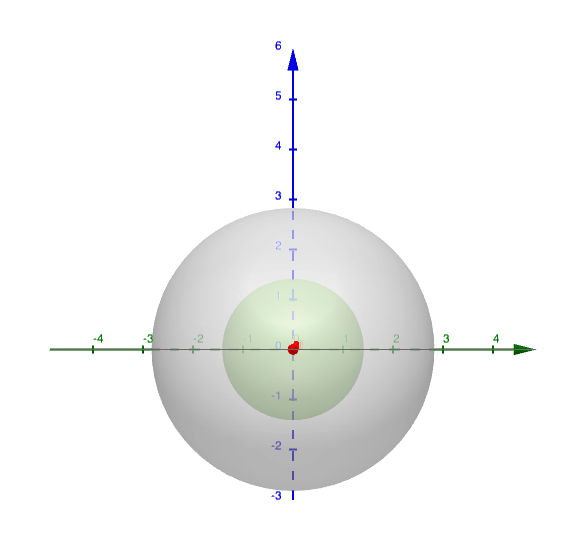
\includegraphics[width=15cm]{Screen Shot 2021-09-27 at 1.04.55 AM.png}
\end{center}
We are observing the region between $a$ and $b$ being two spheres. Therefore, it only makes sense that the integral for the $r$ component is measured from $a$ to $b$. The $\theta$ is measuring the horizontal angle (green line) of the sphere. The sphere contains $2\pi$ of distance; however, if I were to have $2\pi$ for the horizontal and vertical (blue line) then we'd account for more volume then there truly is. That being said, taking the horizontal angle from $0$ to $\pi$ and leaving the vertical angle from $0$ to $2\pi$ so that there isn't any extra volume accounted for.

\newpage
\section*{Question 3c}
\[I=\int\int\int k(x^2+y^2)dV\]
\[\int^{2\pi}_0\int^{\pi}_0\int^{b}_ak(r^2\sin^2\theta\cos^2\phi+r^2\sin^2\theta\sin^2\phi)r^2\sin\theta dr d\theta d\phi\]
\[=\int^{2\pi}_0\int^{\pi}_0\int^{b}_a kr^4\sin^3\theta(\cos^2\phi + \sin^2\phi)dr d\theta d\phi=\int^{2\pi}_0\int^{\pi}_0\int^{b}_a kr^4\sin^3\theta dr d\theta d\phi\]
\[=\frac{(b^5-a^5)k}{5}\int^{2\pi}_0\int^{\pi}_0 \sin^3\theta d\theta d\phi\]
\[\int \sin^3\theta d\theta d\phi=\int (1-\cos^2\theta)\sin\theta d\theta d\phi\]
use the substitution on cos and proceed to use the power rule.
\[=\frac{\cos^3\theta-3\cos\theta}{3}\]
\[=\frac{(b^5-a^5)k}{5}\int^{2\pi}_0 \frac{4}{3} d\phi=\frac{4(b^5-a^5)k}{15}[2\pi]=
\frac{8\pi(b^5-a^5)k}{15} \]
\end{document}
